\clearpage
\subsubsectionold{\olly + упаковка полей по умолчанию}
\myindex{\olly}

Попробуем в \olly наш пример, где поля выровнены по умолчанию (4 байта):

\begin{figure}[H]
\centering
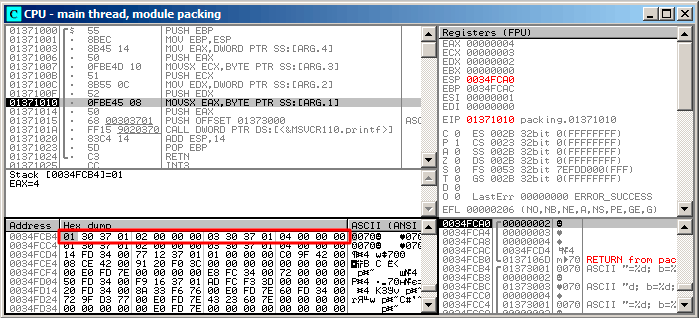
\includegraphics[scale=\FigScale]{patterns/15_structs/4_packing/olly_packing_4.png}
\caption{\olly: Перед исполнением \printf}
\label{fig:packing_olly_4}
\end{figure}

В окне данных видим наши четыре поля.
Вот только, откуда взялись случайные байты (0x30, 0x37, 0x01) рядом с первым (a) и третьим (c) полем?

Если вернетесь к листингу \myref{src:struct_packing_4}, то увидите, что первое и третье поле имеет
тип \Tchar, а следовательно, туда записывается только один байт, 1 и 3 соответственно (строки 6 и 8).

Остальные три байта 32-битного слова не будут модифицироваться в памяти!

А, следовательно, там остается случайный мусор.
\myindex{x86!\Instructions!MOVSX}
Этот мусор никак не будет влиять на работу \printf,
потому что значения для нее готовятся при помощи инструкции \MOVSX, которая загружает
из памяти байты а не слова: 
\lstref{src:struct_packing_4} (строки 34 и 38).

Кстати, здесь используется именно \MOVSX (расширяющая знак), потому что тип 
\Tchar --- знаковый по умолчанию в MSVC и GCC.

Если бы здесь был тип \TT{unsigned char} или \TT{uint8\_t}, 
то здесь была бы инструкция \MOVZX.

\clearpage
\subsubsectionold{\olly + упаковка полей по границе в 1 байт}
\myindex{\olly}

Здесь всё куда понятнее: 4 поля занимают 10 байт и значения сложены в памяти друг к другу

\begin{figure}[H]
\centering
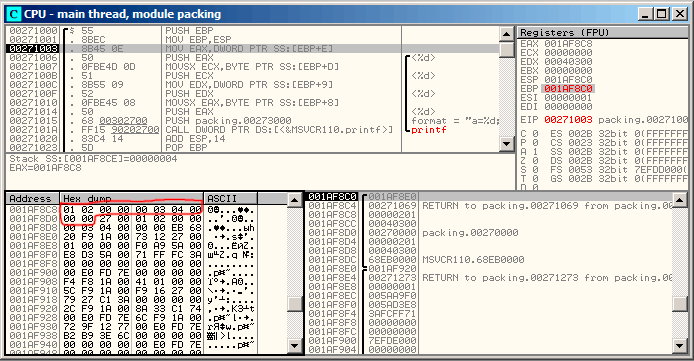
\includegraphics[scale=\FigScale]{patterns/15_structs/4_packing/olly_packing_1.png}
\caption{\olly: Перед исполнением \printf}
\label{fig:packing_olly_1}
\end{figure}
